\documentclass[a4paper,kulak]{kulakarticle}

\usepackage[utf8]{inputenc}
\usepackage[dutch]{babel}
\usepackage{pdfpages}
\usepackage{subfig}
\usepackage{float}

\usepackage{cite}

% style
%\usepackage[left=2.5cm,top=2cm,right=2.5cm,bottom=2cm,a4paper]{geometry}
\usepackage{color}

\date{\today}
\address{
	Bachelor in de fysica\\
	Bachelor in de informatica\\
	Bachelor in de wiskunde\\
	Ingenieurswetenschappen}
\title{BDA App}
\author{Marthe B\"{o}ting\\
	Robin Bruneel\\
	Toon Ingelaere}

\begin{document}
	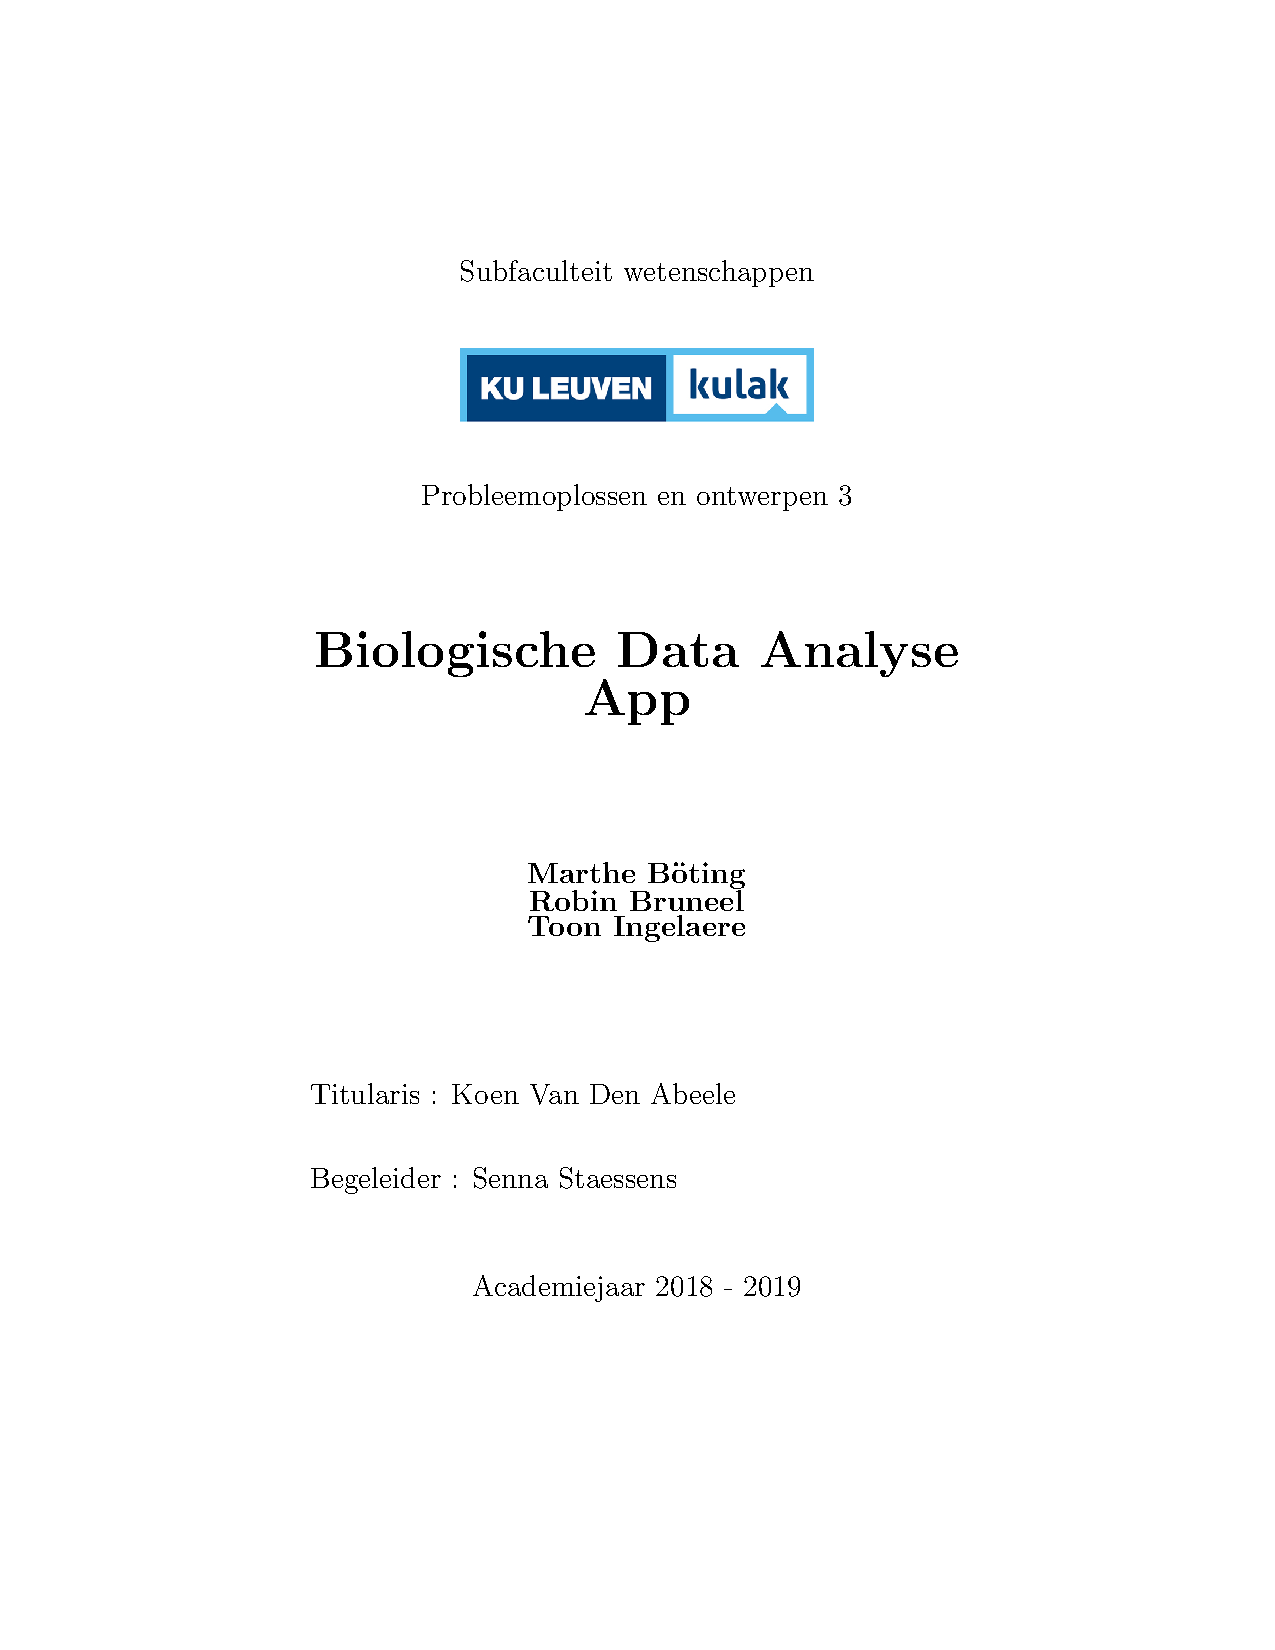
\includepdf{voorblad}
	
	\maketitle

\section*{Inleiding}

Beroertes zijn in onze westerse samenleving de derde grootste doodsoorzaak na hartinfarcten en kanker. Zoals we zien op Figuur \ref{figuur doodsoorzaken} kapen ze op wereldvlak zelfs de tweede plaats weg\cite{worldhealthorganization}. In België komen er gemiddeld 25 000 beroertes per jaar voor. In 15\% van deze gevallen overlijdt de patiënt. De overige 85\% heeft na een beroerte vaak last van blijvende functiebeperkingen zoals cognitieve-, emotionele of gedragsproblemen. Een ischemische beroerte ontstaat doordat een bloedklonter emboliseert en in één van de hersenbloedvaten vast komt te zitten. Deze bloedklonter moet verwijderd worden of de patiënt loopt een hersenschade op.
Momenteel focust de huidige therapie zich op snel en efficiënt verwijderen van de bloedklonter. In eerste instantie kan men via een geneesmiddel, weefsel plasminogeen activator, proberen om de klonter op te lossen. Dit geneesmiddel moet gegeven worden binnen de eerste 4,5 uur na het optreden van de symptomen. Wanneer dit geneesmiddel wordt toegediend na dit tijdstip kan dit leiden tot bloedingen of toxiciteit in de hersenen. Van alle patiënten die het geneesmiddel toegediend krijgen, lost de klonter slechts in 1/3 van de patiënten op.
Op het moment dat de klonter niet oplost , maakt men gebruik van trombectomie om de klonter er manueel uit te halen.
Om huidige therapeutische opties te verbeteren en om het aantal slachtoffers aan beroertes te doen slinken, gebruikt men deze bloedklonters om verder onderzoek op uit te voeren. Hiervoor gaan ze de samenstelling van de bloedklonter proberen te analyseren. Dit gebeurt op basis van afbeeldingen die gemaakt zijn van de bloedklonter waarbij welbepaalde componenten gekleurd zijn (bijvoorbeeld: rode bloedcellen, witte bloedcellen en bloedplaatjes) en vervolgens geanalyseerd worden via kleur-gebaseerde segmentatie analyse.
Deze analyses zijn echter erg tijdrovend. Er is ons dan ook gevraagd om een gebruiksvriendelijke app te ontwikkelen die de analyse van de afbeeldingen kan automatiseren.
In dit verslag gaan we eerst in op wat de klant specifiek van ons verwacht en aan welke specificaties ons ontwerp moet voldoen. Hierna bespreken we ons design en lichten we het toe. Verder bespreken we ook enkele van onze voorlopige resultaten. Ten slotte wordt er nog een blik geworpen naar de vakken uit eerste drie semesters die ons hierbij geholpen hebben.

	\begin{figure}[H]
		\centering
		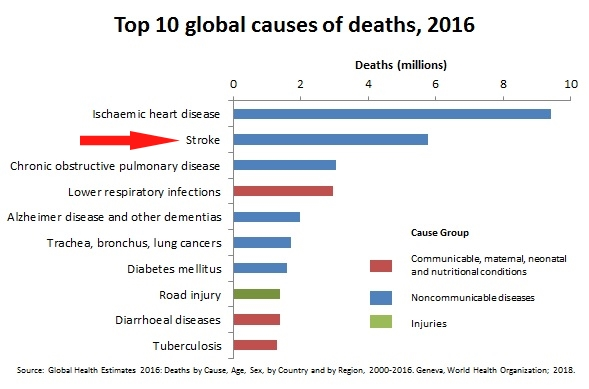
\includegraphics[width = 0.7\textwidth]{top10doodsoorzaken.png}
	
		\caption{Statistieken van de \textit{World Health Organization} van 2016 waarin te zien is dat wereldwijd beroertes (\textit{strokes}) de tweede meest frequente doodsoorzaak is.}
		\label{figuur doodsoorzaken}
	\end{figure}

\pagebreak

%\tableofcontents

\section{Sectie-titel}


Tekst.

\section{De gebruiksvriendelijke applicatie}
De app werkt op basis van de klant die een foto kan ingeven. Het resultaat is een bewerkte foto waarbij er een percentage van de hoeveelheid aanwezig kleur weergegeven wordt.\\
Op het moment dat de klant een afbeelding gekozen heeft, zal  in de eerste fase de achtergrond van de foto wit worden gemaakt en wordt de foto bijgesneden zodanig dat enkel de bloedklonter zichtbaar is. Als dit gebeurd is, zal er al een eerste resultaat getoond worden. Hierdoor heeft de klant een beeld waarop de verdere analyse zal gebeuren en kan die eventueel ingrijpen bij fouten. \\
Vervolgens zal de kleurenanalyse gebeuren. Ook hiervoor zal de foto getoond worden waarop de klant kan zien welke delen de indicator bevatten en zal het percentage gegeven worden. \\
Soms is de kleuring intenser dan anders dit is het gevolg van verschillende factoren (bijvoorbeeld: temperatuur, druk, vochtigheid,... ). Hierdoor kan het resultaat die wordt bekomen via de app eens afwijken van de werkelijke waarde. Daarom hebben wij sliders toegevoegd. Zoals eerder vermeld hebben wij experimenteel waarden bepaald waartussen gewerkt wordt. Door het toevoegen van deze sliders kan de klant zelf deze waarden aanpassen wanneer de kleuring afwijkt. Deze kunnen ook gebruikt worden op het moment dat de bewerkte foto .
Daarnaast is er de mogelijkheid aan om niet foto per foto in te geven maar een volledige map met foto's die dan elk afzonderlijk bewerkt en opgeslagen worden.

\section*{Besluit}

Afsluitende tekst

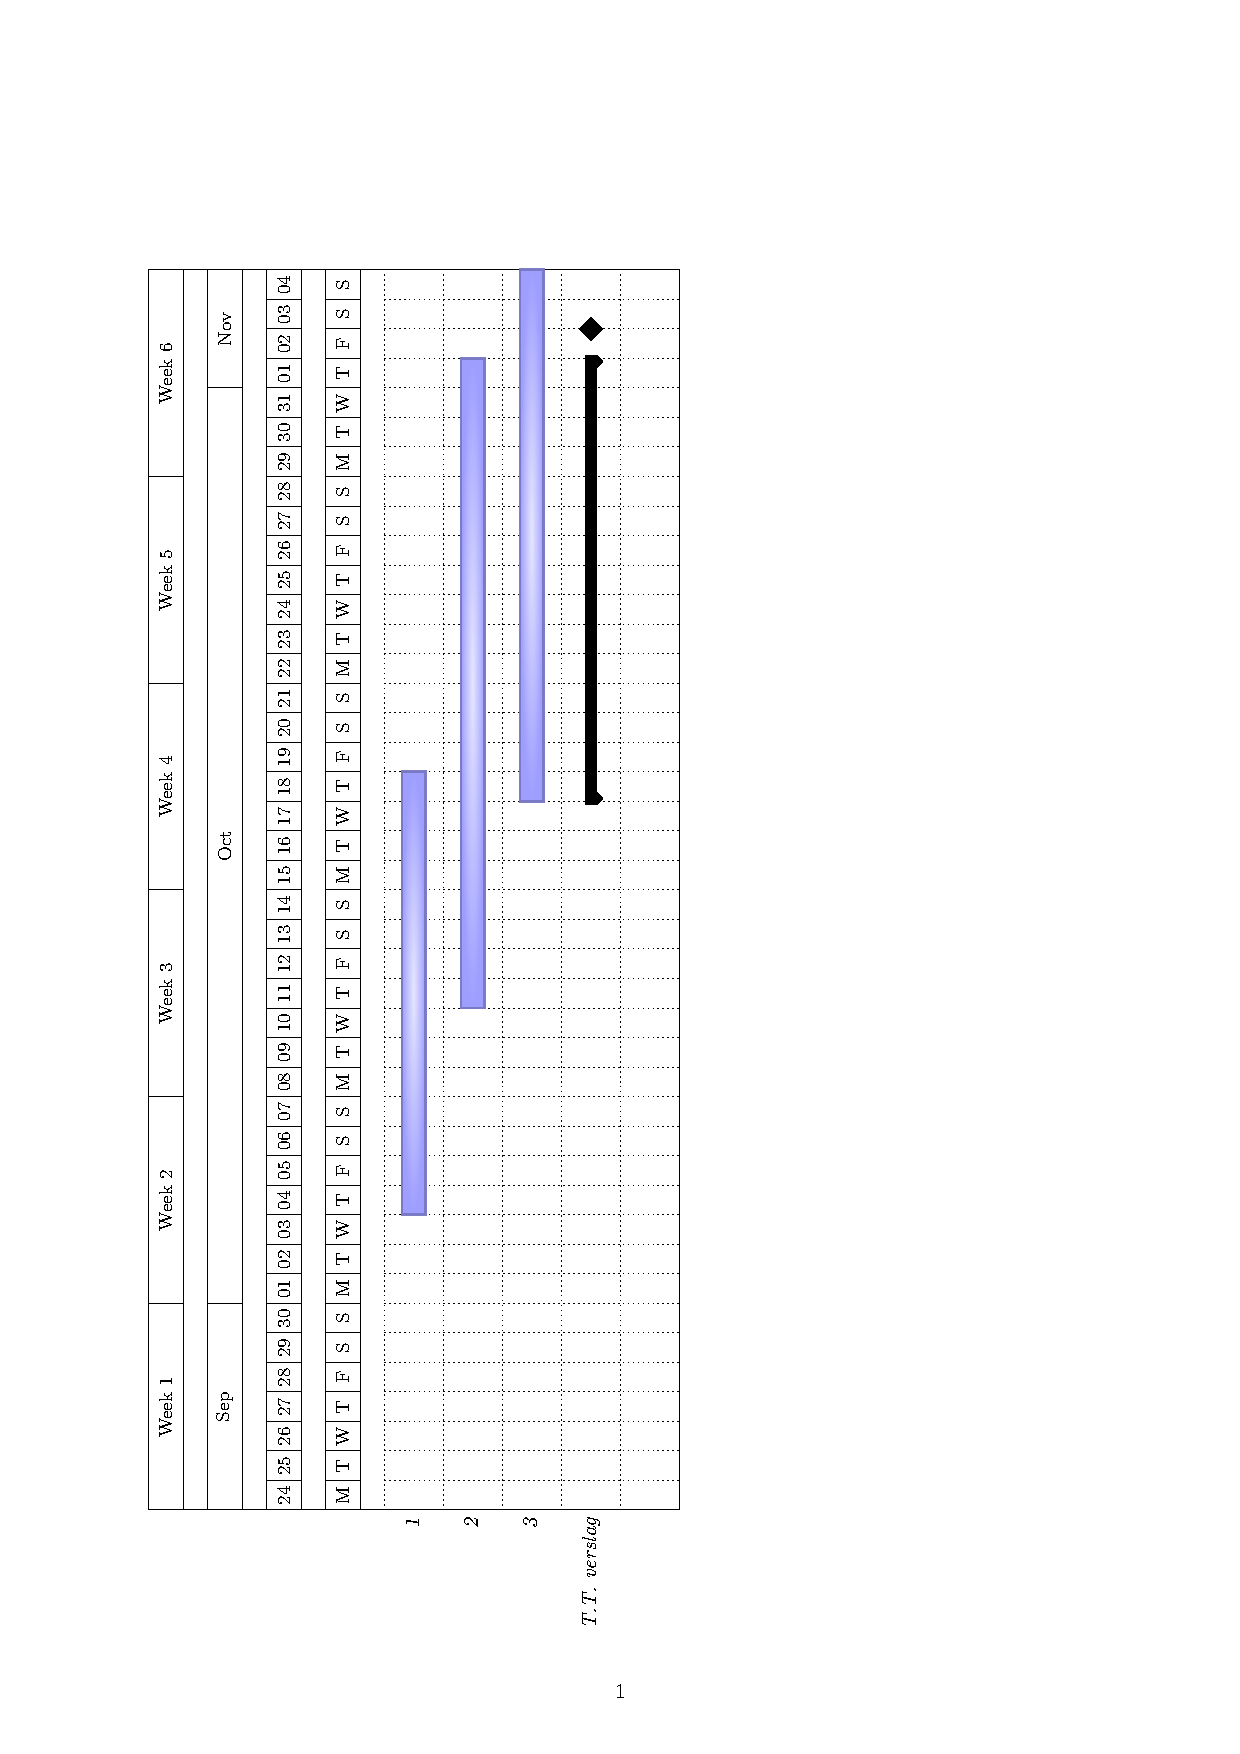
\includepdf[pages={1-3}]{ganttchart}

\end{document}
